\documentclass{article}
\usepackage[utf8]{inputenc}
\usepackage[spanish]{babel}
\usepackage{algorithm}
\usepackage{algpseudocode}
\usepackage{amsmath}
\usepackage{amsfonts}
\usepackage{amssymb}
\usepackage{amsthm}
\usepackage{bm}
\usepackage{float}
\usepackage{forest}
\usepackage{graphicx}
\usepackage{hyperref}
\usepackage{lipsum}
\usepackage{listings}
\usepackage{ragged2e}
\usepackage{url}
\usepackage{xcolor}
\usepackage[T1]{fontenc}
% \usepackage{mathrsfs}
%\usepackage{tikz}
\usepackage{verbatim} % Bloque de comentarios
\usepackage[top=1in, left=1.25in, right=1.25in, bottom=1in]{geometry}

\title{Examen 3, Compiladores}
\author{
Bernal Núñez Raúl \\
Cureño Sanchez Misael
}
\date{Fecha límite de entrega: Martes 14 de noviembre a las 23:59.}

\begin{document}
\maketitle
\begin{enumerate}
    \item (25 pts.) Dada la siguiente gramática:
    
    $$E \quad \rightarrow \quad (E + T) \quad | \quad \textit{id} $$
    $$T \quad \rightarrow \quad (T * F) \quad | \quad \textit{id} $$
    $$F \quad \rightarrow \quad \textit{id} $$
    
    \begin{enumerate}
        \item Construir el \textit{AFD} y la tabla de análisis para un analizador \textit{LR(0)}.
        \begin{proof}[\textbf{Solución: }]
            \quad \\

            Primero es necesario modificar la gramática para agregar una nueva producción: $S \rightarrow E$, donde $S$ es nuestro símbolo inicial.\\

            $S \rightarrow E$\\
            $E  \rightarrow  (E + T)\  |\  \textit{id} $\\
            $T  \rightarrow  (T * F)\  |\  \textit{id} $\\
            $F  \rightarrow  \textit{id} $\\

            Tenemos los siguientes elementos $LR(0)$:\\

            $S \rightarrow .E$\\
            $S \rightarrow E.$\\
            $E \rightarrow .(E+T)$\\
            $E \rightarrow (.E+T)$\\
            $E \rightarrow (E.+T)$\\
            $E \rightarrow (E+.T)$\\
            $E \rightarrow (E+T.)$\\
            $E \rightarrow (E+T).$\\
            $E \rightarrow .id$\\
            $E \rightarrow id.$\\
            $T \rightarrow .(T*F)$\\
            $T \rightarrow (.T*F)$\\
            $T \rightarrow (T.*F)$\\
            $T \rightarrow (T*.F)$\\
            $T \rightarrow (T*F.)$\\
            $T \rightarrow (T*F).$\\
            $T \rightarrow .id$\\
            $T \rightarrow id.$\\
            $F \rightarrow .id$\\
            $F \rightarrow id.$\\


            Ahora vamos a construir directamente el $AFD$: \\
            
            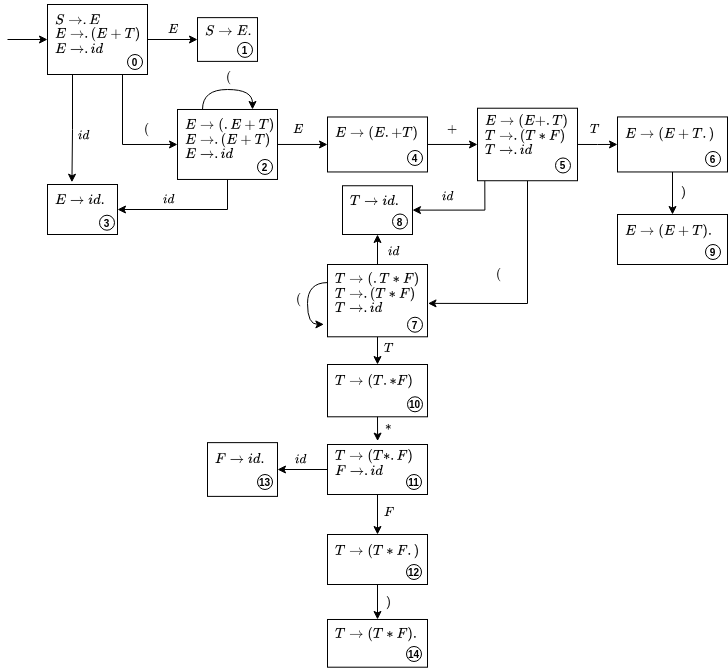
\includegraphics[scale=0.5]{Ej1AFD.png} \\

            La idea es que empezamos con el primer estado que tendrá las producciones de $S$ y $E$ donde el punto está al principio como podemos observar en el estado $0$. Asimismo, de cada estado se van a generar las transiciones a partir del símbolo que esté después del punto en las respectivas producciones del estado, como en el estado $0$ donde tiene tres producciones y se generan tres transiciones con $E$, $($ e $id$ que son los terminales o no terminales a la derecha del punto. \\
            
            Finalmente, el nuevo estado que se genera a través de dichas transiciones siempre va a contener la respectiva producción en la cual el punto se movió un símbolo a la derecha, por ejemplo, estando en el estado $0$ si vemos la segunda producción $E \rightarrow .(E+T)$, se genera la transición con $($ y el nuevo estado, en este caso $2$, tendrá la producción donde el punto aparece después de $($, es decir, $E \rightarrow (.E+T)$. \\

            Sin embargo, tenemos que verificar que si el nuevo estado generado con la producción que difiere únicamente en el punto recorrido a la derecha, tiene el punto antes de un no terminal, entonces tenemos que agregar al estado todas las producciones de dicho no terminal, pero donde el punto está al principio. Lo anterior lo podemos notar con el estado $2$ el cual se genera con $E \rightarrow (.E+T)$, pero después del punto está el no terminal $E$ provocando que se tengan que agregar las producciones de $E$ que tienen el punto al principio al estado $2$. \\

            Siguiendo las ideas anteriores, nos queda el AFD y con eso ya podemos generar nuestra tabla de análisis sintáctico para un analizador $LR(0)$, donde las transiciones nos ayudarán a completar las acciones de desplazamiento y las columnas de los no terminales para saber a qué estado ir. Asimismo, los estados que tienen un elemento completo nos ayudarán a completar las acciones de reducción: \\


            \resizebox{0.9\textwidth}{!}{
            \begin{tabular}{|c|c|c|c|c|c|c|c|c|c|}
              \hline
               & $($ & $)$ & $+$ & $*$ & $id$ & $\$$ & $E$ & $T$ & $F$ \\ \hline
              $0$ & $D-2$ &  &  &  & $D-3$ &  & $1$ &  &  \\ \hline
              $1$ &  &  &  &  &  & $Aceptar$ &  &  &  \\ \hline
              $2$ & $D-2$ &  &  &  & $D-3$ &  & $4$ &  &  \\ \hline
              $3$ & $R: E \rightarrow id$ & $R: E \rightarrow id$ & $R: E \rightarrow id$ & $R: E \rightarrow id$ & $R: E \rightarrow id$ & $R: E \rightarrow id$ &  &  &  \\ \hline
              $4$ &  &  & $D-5$ &  &  &  &  &  &  \\ \hline
              $5$ & $D-7$ &  &  &  & $D-8$ &  &  & $6$ &  \\ \hline
              $6$ &  & $D-9$ &  &  &  &  &  &  &  \\ \hline
              $7$ & $D-7$ &  &  &  & $D-8$ &  &  & $10$ &  \\ \hline
              $8$ & $R: T \rightarrow id$ & $R: T \rightarrow id$ & $R: T \rightarrow id$ & $R: T \rightarrow id$ & $R: T \rightarrow id$ & $R: T \rightarrow id$ &  &  &  \\ \hline
              $9$ & $R: E \rightarrow (E+T)$ & $R: E \rightarrow (E+T)$ & $R: E \rightarrow (E+T)$ & $R: E \rightarrow (E+T)$ & $R: E \rightarrow (E+T)$ & $R: E \rightarrow (E+T)$ &  &  &  \\ \hline
              $10$ &  &  &  & $D-11$ &  &  &  &  &  \\ \hline
              $11$ &  &  &  &  & $D-13$ &  &  &  & $12$ \\ \hline
              $12$ &  & $D-14$ &  &  &  &  &  &  &  \\ \hline
              $13$ & $R: F \rightarrow id$ & $R: F \rightarrow id$ & $R: F \rightarrow id$ & $R: F \rightarrow id$ & $R: F \rightarrow id$ & $R: F \rightarrow id$ &  &  &  \\ \hline
              $14$ & $R: T \rightarrow (T * F)$ & $R: T \rightarrow (T * F)$ & $R: T \rightarrow (T * F)$ & $R: T \rightarrow (T * F)$ & $R: T \rightarrow (T * F)$ & $R: T \rightarrow (T * F)$ &  &  &  \\ \hline
            \end{tabular}
            }
            \vspace{10pt}

            Finalmente, podemos ver que la gramática proporcionada es $LR(0)$ pues se logró generar la tabla de análisis sintáctica de manera correcta sin conflictos. \\
        \end{proof}
        
        \item Construir el \textit{AFD} y la tabla de análisis para un analizador \textit{SLR(1)}.
        \begin{proof}[\textbf{Solución: }]
            \quad \\

            Para este inciso podemos reutilizar el autómata que generamos para el analizador $LR(0)$: \\

            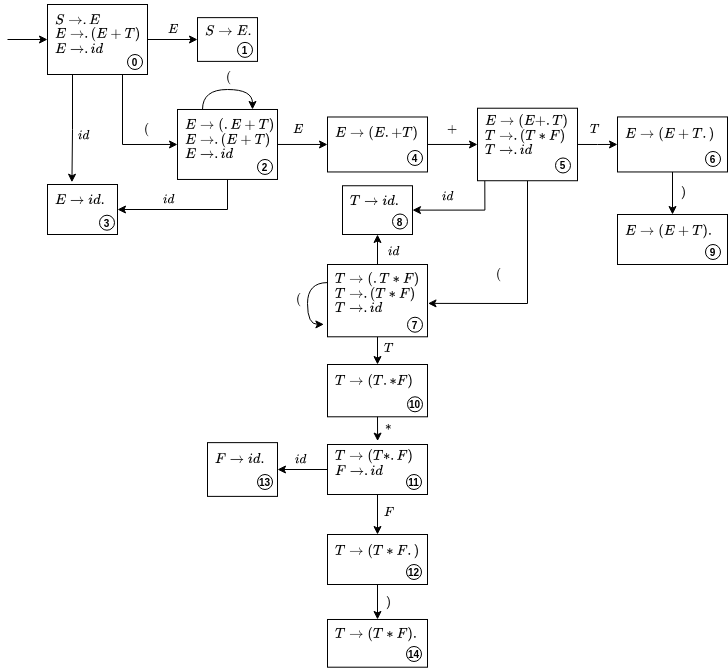
\includegraphics[scale=0.5]{Ej1AFD.png}

            La diferencia es que ahora necesitaremos calcular los conjuntos Siguiente de la gramática:

            \begin{align*}
                Siguiente(S) & = \{\$\} \\
                Siguiente(E) & = \{\$, +\} \\
                Siguiente(T) & = \{), *\} \\
                Siguiente(F) & = \{)\}
            \end{align*}

            Con ayuda del autómata y de los conjuntos Siguiente generamos la tabla de análisis sintáctico, donde se realizará lo mismo que para $LR(0)$ con la diferencia de que las casillas en las que se añadirá la producción que nos indica cómo reducir será únicamente en las columnas correspondientes a los respectivos elementos de los conjuntos Siguiente: \\

            \resizebox{0.9\textwidth}{!}{
            \begin{tabular}{|c|c|c|c|c|c|c|c|c|c|}
              \hline
               & $($ & $)$ & $+$ & $*$ & $id$ & $\$$ & $E$ & $T$ & $F$ \\ \hline
              $0$ & $D-2$ &  &  &  & $D-3$ &  & $1$ &  &  \\ \hline
              $1$ &  &  &  &  &  & $Aceptar$ &  &  &  \\ \hline
              $2$ & $D-2$ &  &  &  & $D-3$ &  & $4$ &  &  \\ \hline
              $3$ &  &  & $R: E \rightarrow id$ &  &  & $R: E \rightarrow id$ &  &  &  \\ \hline
              $4$ &  &  & $D-5$ &  &  &  &  &  &  \\ \hline
              $5$ & $D-7$ &  &  &  & $D-8$ &  &  & $6$ &  \\ \hline
              $6$ &  & $D-9$ &  &  &  &  &  &  &  \\ \hline
              $7$ & $D-7$ &  &  &  & $D-8$ &  &  & $10$ &  \\ \hline
              $8$ &  & $R: T \rightarrow id$ &  & $R: T \rightarrow id$ &  &  &  &  &  \\ \hline
              $9$ &  &  & $R: E \rightarrow (E+T)$ &  &  & $R: E \rightarrow (E+T)$ &  &  &  \\ \hline
              $10$ &  &  &  & $D-11$ &  &  &  &  &  \\ \hline
              $11$ &  &  &  &  & $D-13$ &  &  &  & $12$ \\ \hline
              $12$ &  & $D-14$ &  &  &  &  &  &  &  \\ \hline
              $13$ &  & $R: F \rightarrow id$ &  &  &  &  &  &  &  \\ \hline
              $14$ &  & $R: T \rightarrow (T * F)$ &  & $R: T \rightarrow (T * F)$ &  &  &  &  &  \\ \hline
            \end{tabular}
            }
            \vspace{10pt}

        Finalmente, podemos ver que la gramática proporcionada es también $SLR(1)$ pues se logró generar la tabla de análisis sintáctica de manera correcta sin conflictos. \\
        \end{proof}
        
        \item Reconocer la cadena $(6 + (4 * 2))$ con ambos analizadores.
        \definecolor{green}{RGB}{15,130,35}
        \begin{proof}[\textbf{Solución: }]
            \quad \\

            \textit{Nota: Los símbolos 6, 4 y 2, los vamos a considerar como terminales $id$.}\\
            
            Utilizando nuestro analizador $LR(0)$: \\

            \resizebox{0.85\textwidth}{!}{
                \begin{tabular}{|c|c|c|c|c|}
                    \hline
                    Paso & Pila de análisis sintáctico & Entrada & Acción a aplicar \\ \hline
                    1 & $\$\ 0$  & $\textcolor{green}{(6 + (4 * 2))} \$$ & $D-2$ \\ \hline
                    2 & $\$\ 0\ \textcolor{green}{(}\ 2$  & $\textcolor{green}{6 + (4 * 2))} \$$ & $D-3$ \\ \hline
                    3 & $\$\ 0\ \textcolor{green}{(}\ 2\ \textcolor{green}{6}\ 3$  & $\textcolor{green}{ + (4 * 2))} \$$ & $R: E \rightarrow id$ \\ \hline
                    4 & $\$\ 0\ \textcolor{green}{(}\ 2\ \textcolor{green}{E}\ 4$  & $\textcolor{green}{ + (4 * 2))} \$$ & $D-5$ \\ \hline
                    5 & $\$\ 0\ \textcolor{green}{(}\ 2\ \textcolor{green}{E}\ 4\ \textcolor{green}{+}\ 5$  & $\textcolor{green}{(4 * 2))} \$$ & $D-7$ \\ \hline
                    6 & $\$\ 0\ \textcolor{green}{(}\ 2\ \textcolor{green}{E}\ 4\ \textcolor{green}{+}\ 5\ \textcolor{green}{(}\ 7$  & $\textcolor{green}{4 * 2))} \$$ & $D-8$ \\ \hline
                    7 & $\$\ 0\ \textcolor{green}{(}\ 2\ \textcolor{green}{E}\ 4\ \textcolor{green}{+}\ 5\ \textcolor{green}{(}\ 7\ \textcolor{green}{4}\ 8$  & $\textcolor{green}{ *\ 2))} \$$ & $R: T \rightarrow id$ \\ \hline
                    8 & $\$\ 0\ \textcolor{green}{(}\ 2\ \textcolor{green}{E}\ 4\ \textcolor{green}{+}\ 5\ \textcolor{green}{(}\ 7\ \textcolor{green}{T}\ 10$  & $\textcolor{green}{ *\ 2))} \$$ & $D-11$ \\ \hline
                    9 & $\$\ 0\ \textcolor{green}{(}\ 2\ \textcolor{green}{E}\ 4\ \textcolor{green}{+}\ 5\ \textcolor{green}{(}\ 7\ \textcolor{green}{T}\ 10\ \textcolor{green}{*}\ 11$  & $\textcolor{green}{2))} \$$ & $D-13$ \\ \hline
                    10 & $\$\ 0\ \textcolor{green}{(}\ 2\ \textcolor{green}{E}\ 4\ \textcolor{green}{+}\ 5\ \textcolor{green}{(}\ 7\ \textcolor{green}{T}\ 10\ \textcolor{green}{*}\ 11\ \textcolor{green}{2}\ 13$  & $\textcolor{green}{))} \$$ & $R: F \rightarrow id$ \\ \hline
                    11 & $\$\ 0\ \textcolor{green}{(}\ 2\ \textcolor{green}{E}\ 4\ \textcolor{green}{+}\ 5\ \textcolor{green}{(}\ 7\ \textcolor{green}{T}\ 10\ \textcolor{green}{*}\ 11\ \textcolor{green}{F}\ 12$  & $\textcolor{green}{))} \$$ & $D-14$ \\ \hline
                    12 & $\$\ 0\ \textcolor{green}{(}\ 2\ \textcolor{green}{E}\ 4\ \textcolor{green}{+}\ 5\ \textcolor{green}{(}\ 7\ \textcolor{green}{T}\ 10\ \textcolor{green}{*}\ 11\ \textcolor{green}{F}\ 12\ \textcolor{green}{)}\ 14$  & $\textcolor{green}{)} \$$ & $R: T \rightarrow (T * F)$ \\ \hline
                    13 & $\$\ 0\ \textcolor{green}{(}\ 2\ \textcolor{green}{E}\ 4\ \textcolor{green}{+}\ 5\ \textcolor{green}{T}\ 6$  & $\textcolor{green}{)} \$$ & $D-9$ \\ \hline
                    14 & $\$\ 0\ \textcolor{green}{(}\ 2\ \textcolor{green}{E}\ 4\ \textcolor{green}{+}\ 5\ \textcolor{green}{T}\ 6\ \textcolor{green}{)}\ 9$  & $ \$$ & $R: E \rightarrow (E + T)$ \\ \hline
                    15 & $\$\ 0\ \textcolor{green}{E}\ 1$  & $ \$$ & $Aceptar$ \\ \hline
                \end{tabular}
            }
            \vspace{10pt}

            Utilizando ahora nuestro analizador $SLR(1)$: \\

            \resizebox{0.85\textwidth}{!}{
                \begin{tabular}{|c|c|c|c|c|}
                    \hline
                    Paso & Pila de análisis sintáctico & Entrada & Acción a aplicar \\ \hline
                    1 & $\$\ 0$  & $\textcolor{green}{(6 + (4 * 2))} \$$ & $D-2$ \\ \hline
                    2 & $\$\ 0\ \textcolor{green}{(}\ 2$  & $\textcolor{green}{6 + (4 * 2))} \$$ & $D-3$ \\ \hline
                    3 & $\$\ 0\ \textcolor{green}{(}\ 2\ \textcolor{green}{6}\ 3$  & $\textcolor{green}{ + (4 * 2))} \$$ & $R: E \rightarrow id$ \\ \hline
                    4 & $\$\ 0\ \textcolor{green}{(}\ 2\ \textcolor{green}{E}\ 4$  & $\textcolor{green}{ + (4 * 2))} \$$ & $D-5$ \\ \hline
                    5 & $\$\ 0\ \textcolor{green}{(}\ 2\ \textcolor{green}{E}\ 4\ \textcolor{green}{+}\ 5$  & $\textcolor{green}{(4 * 2))} \$$ & $D-7$ \\ \hline
                    6 & $\$\ 0\ \textcolor{green}{(}\ 2\ \textcolor{green}{E}\ 4\ \textcolor{green}{+}\ 5\ \textcolor{green}{(}\ 7$  & $\textcolor{green}{4 * 2))} \$$ & $D-8$ \\ \hline
                    7 & $\$\ 0\ \textcolor{green}{(}\ 2\ \textcolor{green}{E}\ 4\ \textcolor{green}{+}\ 5\ \textcolor{green}{(}\ 7\ \textcolor{green}{4}\ 8$  & $\textcolor{green}{ *\ 2))} \$$ & $R: T \rightarrow id$ \\ \hline
                    8 & $\$\ 0\ \textcolor{green}{(}\ 2\ \textcolor{green}{E}\ 4\ \textcolor{green}{+}\ 5\ \textcolor{green}{(}\ 7\ \textcolor{green}{T}\ 10$  & $\textcolor{green}{ *\ 2))} \$$ & $D-11$ \\ \hline
                    9 & $\$\ 0\ \textcolor{green}{(}\ 2\ \textcolor{green}{E}\ 4\ \textcolor{green}{+}\ 5\ \textcolor{green}{(}\ 7\ \textcolor{green}{T}\ 10\ \textcolor{green}{*}\ 11$  & $\textcolor{green}{2))} \$$ & $D-13$ \\ \hline
                    10 & $\$\ 0\ \textcolor{green}{(}\ 2\ \textcolor{green}{E}\ 4\ \textcolor{green}{+}\ 5\ \textcolor{green}{(}\ 7\ \textcolor{green}{T}\ 10\ \textcolor{green}{*}\ 11\ \textcolor{green}{2}\ 13$  & $\textcolor{green}{))} \$$ & $R: F \rightarrow id$ \\ \hline
                    11 & $\$\ 0\ \textcolor{green}{(}\ 2\ \textcolor{green}{E}\ 4\ \textcolor{green}{+}\ 5\ \textcolor{green}{(}\ 7\ \textcolor{green}{T}\ 10\ \textcolor{green}{*}\ 11\ \textcolor{green}{F}\ 12$  & $\textcolor{green}{))} \$$ & $D-14$ \\ \hline
                    12 & $\$\ 0\ \textcolor{green}{(}\ 2\ \textcolor{green}{E}\ 4\ \textcolor{green}{+}\ 5\ \textcolor{green}{(}\ 7\ \textcolor{green}{T}\ 10\ \textcolor{green}{*}\ 11\ \textcolor{green}{F}\ 12\ \textcolor{green}{)}\ 14$  & $\textcolor{green}{)} \$$ & $R: T \rightarrow (T * F)$ \\ \hline
                    13 & $\$\ 0\ \textcolor{green}{(}\ 2\ \textcolor{green}{E}\ 4\ \textcolor{green}{+}\ 5\ \textcolor{green}{T}\ 6$  & $\textcolor{green}{)} \$$ & $D-9$ \\ \hline
                    14 & $\$\ 0\ \textcolor{green}{(}\ 2\ \textcolor{green}{E}\ 4\ \textcolor{green}{+}\ 5\ \textcolor{green}{T}\ 6\ \textcolor{green}{)}\ 9$  & $ \$$ & $R: E \rightarrow (E + T)$ \\ \hline
                    15 & $\$\ 0\ \textcolor{green}{E}\ 1$  & $ \$$ & $Aceptar$ \\ \hline
                \end{tabular}
            }
            \vspace{10pt}

            Con lo anterior, podemos notar que ambos analizadores aceptan la cadena correspondiente de la misma manera, en este caso no vemos un cambio porque la cadena es válida y además desde la tabla que se utilizó para $LR(0)$ no hubo conflictos, por lo que al hacer la tabla de $SLR(1)$ tampoco existieron conflictos. Sin embargo, si existirán algunos casos cuando una cadena no sea válida donde el analizador $SLR(1)$ se dará cuenta antes de un error. \\
        \end{proof}
    \end{enumerate}

    \item (25 pts.) Indica si los siguientes enunciados son falsos o verdaderos. Justifica tu respuesta.
    \begin{enumerate}
        \item Una gramática \textit{LR(1)} que no es \textit{LALR(1)} debe tener sólo conflictos de reducción-reducción.
        \begin{proof}[\textbf{Solución: }]
            \quad \\ \\
            Si tenemos una gramática $LR(1)$ que no es $LALR(1)$, entonces únicamente debería tener conflictos de desplazamiento-reducción, pues los conflictos de reducción-reducción pueden surgir al momento de simplificar el autómata de $LR(1)$ al autómata de $LALR(1)$, sin embargo, estamos suponiendo que $LR(1)$ no es $LALR(1)$, así dicha simplificación no se da, ocasionando que únicamente se tengan los conflictos de desplazamiento-reducción. Por lo tanto, es falso que una gramática $LR(1)$ que no es $LALR(1)$ debe tener sólo conflictos de reducción-reducción. \\
        \end{proof}
        
        \item Pueden haber gramáticas \textit{SLR(1)} que no sean \textit{LALR(1)}.
        \begin{proof}[\textbf{Solución: }]
            \quad \\ \\
            Considero que no pueden haber gramáticas $SLR(1)$ que no sean $LALR(1)$, pues supongamos que $G_1$ y $G_2$ son gramáticas reconocidas por el autómata de $SLR(1)$ y de $LALR(1)$, respectivamente, entonces tenemos que para generar el autómata de $LALR(1)$ se utiliza en los elementos de cada estado un elemento $LR(0)$ junto con no terminales o $\$$, es decir, usa un elemento $LR(1)$ con la finalidad de que se pueda basar en un token de la entrada para decidir si seguir con el análisis de la cadena o rechazarla. Asimismo, en el autómata de $SLR(1)$ se tienen únicamente los elementos $LR(0)$, y en este caso se ayuda de los conjuntos Siguiente y de un token de la entrada para saber si al momento de reducir, para así evitar realizar una reducción si el token de la entrada no corresponde con lo esperado y así rechazar la cadena de entrada. \\

            Con lo anterior podemos notar que el autómata de $SLR(1)$ lo que hace es evitar mayor número de conflictos con respecto a $LR(0)$, pues puede saber si rechazar una cadena antes de hacer una reducción, para que si no se puede rechace las cadenas no válidas más rápido, pero el autómata de $LALR(1)$ además de verificar si es válido hacer una reducción basado en la entrada y el elemento de un estado, también verifica si es válido realizar un desplazamiento utilizando igualmente el elemento de un estado y un token de la entrada. Por lo tanto, observamos que el autómata de $LALR(1)$ es más poderoso, con lo cual no puede haber una gramática $SLR(1)$ que no sea $LALR(1)$, entonces el enunciado es falso. \\
        \end{proof}
    \end{enumerate}
    
    \item (25 pts) Dada la siguiente gramática con atributos:
    \begin{table}[h]
        \centering
        \begin{tabular}{|l|l|}
            \hline
            $S' \rightarrow S$ & $print(\$1.v)$ \\ \hline
            $S \rightarrow AS$ &
            $
            \begin{array} {lcl}
                \$\$.v & = & \$1.v \\
                \$1.x & = & \$2.v
            \end{array}
            $ \\ \hline
            $S \rightarrow A$ &
            $
            \begin{array} {lcl}
                \$1.x & = & 0 \\
                \$\$.v & = & \$1.v
            \end{array}
            $ \\ \hline
            $A \rightarrow a$  & $
            \begin{array} {lcl}
                \$\$.v & = & \$\$.x + 1
            \end{array}
            $ \\ \hline
        \end{tabular}
    \end{table}
    
    \begin{enumerate}
        \item Mostrar el árbol sintáctico (gramatical o \textit{ASA}) decorado para la cadena de entrada \textit{aaaa} e indicar la salida que provoca el análisis semántico.
        \begin{proof}[\textbf{Solución: }]
            \quad \\
            \begin{center}
                \begin{forest}
                [S'
                    [S
                        [A  [a]] {
                            \draw[<-,red] (.south west)--++(0em,-1ex)--++(-4em,0pt) node[anchor=east]{
                                $\{\$\$.v = \$\$.x + 1 = 3 + 1 = 4,\quad \$\$.x = 3\}$
                            };
                        }
                        [S
                            [A  [a]] {
                                \draw[<-,red] (.south west)--++(0em,-1ex)--++(-4em,0pt) node[anchor=east]{
                                    $\{\$\$.v = \$\$.x + 1 = 2 + 1 = 3,\quad \$\$.x = 2\}$
                                };
                            }
                            [S
                                [A  [a]] {
                                    \draw[<-,red] (.south west)--++(0em,-1ex)--++(-4em,0pt) node[anchor=east]{
                                        $\{\$\$.v = \$\$.x + 1 = 1 + 1 = 2,\quad \$\$.x = 1\}$
                                    };
                                }
                                [S
                                    [A  [a]] {
                                        \draw[<-,red] (.south west)--++(0em,-1ex)--++(-4em,0pt) node[anchor=east]{
                                            $\{\$\$.v = \$\$.x + 1 = 0 + 1 = 1,\quad \$\$.x = 0\}$
                                        };
                                    }
                                ] {
                                    \draw[<-,cyan] (.east)--++(2em,0pt) node[anchor=west]{
                                        $\{\$\$.v = 1\}$
                                    };
                                }
                            ] {
                                \draw[<-,cyan] (.east)--++(2em,0pt) node[anchor=west]{
                                    $\{\$\$.v = 2\}$
                                };
                            }
                        ] {
                            \draw[<-,cyan] (.east)--++(2em,0pt) node[anchor=west]{
                                $\{\$\$.v = 3\}$
                            };
                        }
                    ] {
                        \draw[<-,cyan] (.east)--++(2em,0pt) node[anchor=west]{
                            $\{\$\$.v = 4\}$
                        };
                    }
                ] {
                    \draw[<-,cyan] (.east)--++(2em,0pt) node[anchor=west]{
                        $print(4)$
                    };
                }
                \end{forest}
            \end{center}
            Al realizar el árbol notamos que la gramática con atributos proporcionada sirve para contar la cantidad de $a's$, y en la cadena proporcionada hay 4 $a's$, y la salida que provoca el análasis semántico es 4, por lo tanto, el análisis es correcto. \\
        \end{proof}
    \end{enumerate}

    \item (25 pts) Dada la siguiente gramática que genera números binarios:
    
    $$ \quad A \rightarrow \quad AB \quad | \quad B$$
    $$ \quad B \rightarrow \quad 0 \quad | \quad 1$$
    
    \begin{enumerate}
        \item Obtener la gramática con atributos que al analizar un número binario calcule su equivalente en decimal.
        \begin{proof}[\textbf{Solución: }]
            \quad \\
            \begin{table}[h]
                \centering
                \begin{tabular}{|l|l|} 
                    \hline
                    $A' \rightarrow A$ & $print(\$1.v)$ \\ \hline
                    $A \rightarrow AB$ &
                    $
                    \begin{array} {lcl}
                        \$\$.v & = & 2 * (\$1.v) + \$2.v
                    \end{array}
                    $ \\ \hline
                    $A \rightarrow B$ &
                    $
                    \begin{array} {lcl}
                        \$\$.v & = & \$1.v
                    \end{array}
                    $ \\ \hline
                    $B \rightarrow 0 \text{ } | \text{ } 1$ &
                    $
                    \begin{array} {lcl}
                        \$\$.v & = & 0 \text{ } | \text{ } 1
                    \end{array}
                    $ \\ \hline
                \end{tabular}
            \end{table}
            \hspace{0pt} \\
        \end{proof}
        
        \item Mostrar el árbol para la cadena de entrada 101 e indicar la salida que provoca el análisis semántico.
        \begin{proof}[\textbf{Solución: }]
            \quad \\ \\
            Árbol de sintaxis abstracta:
            \begin{center}
                \begin{forest}
                [A'
                    [A
                        [A
                            [A
                                [B  [1]] {
                                    \draw[<-,red] (.south east)--++(0em,-1ex)--++(4em,0pt) node[anchor=west]{
                                        $\{\$\$.v = 1\}$
                                    };
                                }
                            ] {
                                \draw[<-,cyan] (.west)--++(-2em,0pt) node[anchor=east]{
                                    $\{\$\$.v = \$1.v = 1\}$
                                };
                            }
                            [B  [0]] {
                                \draw[<-,red] (.south east)--++(0em,-1ex)--++(4em,0pt) node[anchor=west]{
                                    $\{\$\$.v = 0\}$
                                };
                            }
                        ] {
                            \draw[<-,cyan] (.west)--++(-2em,0pt) node[anchor=east]{
                                $\{\$\$.v = 2 * (\$1.v) + \$2.v = 2 * (1) + 0 = 2\}$
                            };
                        }
                        [B  [1]] {
                            \draw[<-,red] (.south east)--++(0em,-1ex)--++(4em,0pt) node[anchor=west]{
                                $\{\$\$.v = 1\}$
                            };
                        }
                    ] {
                        \draw[<-,cyan] (.west)--++(-2em,0pt) node[anchor=east]{
                            $\{\$\$.v = 2 * (\$1.v) + \$2.v = 2 * (2) + 1 = 5\}$
                        };
                    }
                ] {
                    \draw[<-,cyan] (.west)--++(-2em,0pt) node[anchor=east]{
                        $print (5)$
                    };
                }
                \end{forest}
            \end{center}
            La gramática del inciso $a)$, sirve para calcular el número en decimal correspondiente al binario proporcionado, y la cadena proporcionada es 101 que en decimal tiene un valor de 5, y la salida que provoca el análasis semántico es 5, por lo tanto, el análisis es correcto. \\
        \end{proof}
    \end{enumerate}
\end{enumerate}

\end{document}